\documentclass{../bredelebeamer}
\usepackage{multirow}
\usepackage{pdfpages}
\usepackage{braket,bigstrut}
\usepackage{palatino}
\usepackage{multicol,bigstrut}
\usepackage{listings}
\usepackage{tikz}
\usepackage{pgfplots}
\pgfplotsset{compat=1.17}
\usepackage{booktabs}
\usepackage{amsmath,amssymb,amsfonts,cancel,physics,siunitx}
\usetikzlibrary{positioning,shadows,backgrounds,calc}%
\setbeamercolor{footnote mark}{fg=black}
\setbeamercolor{footnote}{fg=black}


\renewcommand{\baselinestretch}{0.9}

\usepackage[backend=bibtex8,style=authortitle,autocite=footnote]{biblatex}
\addbibresource{referencia.bib}

\renewbibmacro*{cite:title}{%
	\printtext[bibhyperref]{%
		\printfield[citetitle]{labeltitle}%
		\setunit{\space}%
		\printtext[parens]{\printdate}%
	}%
}
\renewcommand{\figurename}{{\bf Fig.}}
\usefonttheme{serif} % default family is serif

\renewcommand{\baselinestretch}{0.9}

\title[THDM - PUCP Internship 2025]{Two Higgs Doublet Model(s)}
\subtitle{}
\author[C. Rodríguez]{%
    \vspace{2em}\\
    PhD(c). Cristian Fernando Rodríguez Cruz\inst{1}\\
    \href{mailto:c.rodriguez45@uniandes.edu.co}{c.rodriguez45@uniandes.edu.co}\\
    \vspace{1em}
    Research advisors:\\
    \vspace{0.5em}
    Prof. Andrés Florez\inst{1} ( \href{mailto:ca.florez@uniandes.edu.co}{ca.florez@uniandes.edu.co} )\\
    \vspace{0.5em}
    Prof. J. Jones-Pérez\inst{2} ( \href{mailto:jones.j@pucp.edu.pe}{jones.j@pucp.edu.pe} )\\
    \vspace{1em}
}

\institute[BSM3G]{\inst{1} Universidad de los Andes\and
\inst{2} Pontificia Universidad Católica del Perú
}
\date{\today}
\lstset{language=C++,
  basicstyle=\ttfamily,
  keywordstyle=\color{blue}\ttfamily,
  stringstyle=\color{red}\ttfamily,
  commentstyle=\color{green}\ttfamily,
  morecomment=[l][\color{magenta}]{\#}
}

\begin{document}
\frame{\titlepage}

\begin{frame}
    \frametitle{Outline}
    \tableofcontents
\end{frame}

\section{Introduction}

\begin{frame}{The Standard Model Higgs Mechanism}
        \begin{center}
            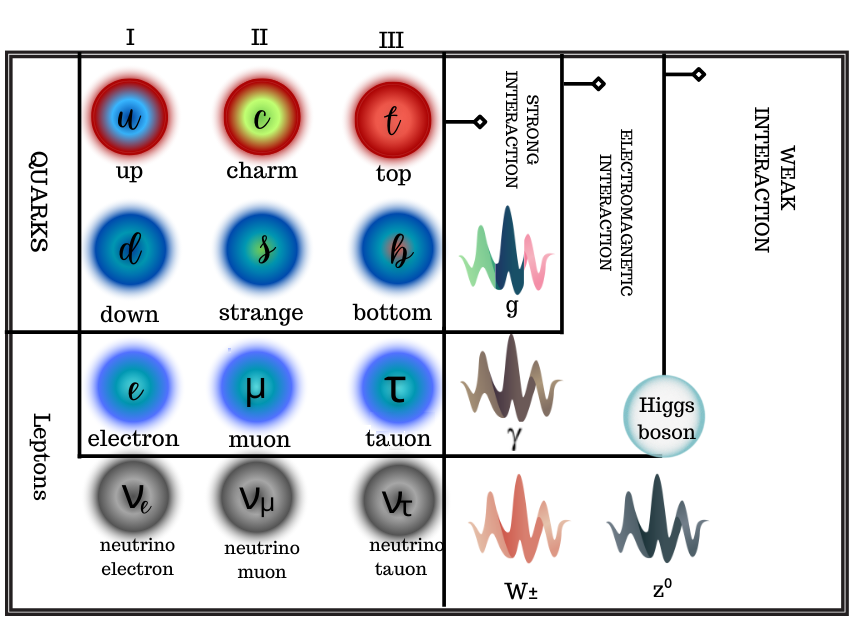
\includegraphics[width=.75\linewidth]{../2023_paper/SM}
        \end{center}
        \begin{itemize}
            \item One Higgs doublet provides EWSB
            \item Single physical Higgs boson discovered in 2012
            \item But is this the complete story?
        \end{itemize}
\end{frame}

\begin{frame}{Why Consider Extended Higgs Sectors?}
    \begin{block}{BSM Motivations}
        \begin{itemize}
            \item \textcolor{blue}{\textbf{Hierarchy Problem}} \\ 
            \small Discrepancy between Higgs mass ($\sim$125 GeV) and Planck scale ($\sim10^{19}$ GeV)
            
            \item \textcolor{blue}{\textbf{Dark Matter Puzzle}} \\ 
            \small No viable DM candidate in SM (WIMP miracle suggests $\sim$100 GeV scale)
            
            \item \textcolor{blue}{\textbf{Baryogenesis Requirements}} \\ 
            \small Need strong 1st-order EW phase transition ($v_c/T_c > 1$)
            
            \item \textcolor{blue}{\textbf{Flavor Anomalies}} \\ 
            \small Additional CP violation sources needed for $B$-physics observations
            
            \item \textcolor{blue}{\textbf{Theoretical Naturalness}} \\ 
            \small SUSY, composite Higgs, etc. often require extended sectors
        \end{itemize}
    \end{block}
    
    \vspace{0.5cm}
    
    \begin{exampleblock}{The Minimal Extension: Two Higgs Doublet Model (2HDM)}
        \centering
        \textbf{Simplest framework} addressing some of these challenges \\ 
        {\footnotesize (Different types: Type I, II, Lepton-specific, Flipped with different phenomenology)}
    \end{exampleblock}
\end{frame}

\section{On the Scalar Potential}

\begin{frame}{Purely Scalar Extension}
    \begin{itemize}
        \item With Two Higgs doublets under $SU(2)_L \times U(1)_Y$, the most general potential is
          {\small
            \begin{align}
              V_{\text {tree }}= 
              &\quad \textcolor{blue!60!black}{m_{11}^2\left(\Phi_1^{\dagger} \Phi_1\right) +\frac{\lambda_1}{2}\left(\Phi_1^{\dagger} \Phi_1\right)^2+ m_{22}^2\left(\Phi_2^{\dagger} \Phi_2\right)
              +\frac{\lambda_2}{2}\left(\Phi_2^{\dagger} \Phi_2\right)^2}\\
              & +\textcolor{purple!80!black}{\lambda_3\left(\Phi_1^{\dagger} \Phi_1\right)\left(\Phi_2^{\dagger} \Phi_2\right)+\lambda_4\left(\Phi_1^{\dagger} \Phi_2\right)\left(\Phi_2^{\dagger} \Phi_1\right) + \frac{1}{2}\left[ \lambda_5\left(\Phi_1^{\dagger} \Phi_2\right)^2 + \text{h.c.}\right]}\\
              & +\textcolor{brown!85!black}{\left[ -m_{12}^2\Phi_1^{\dagger} \Phi_2 +\lambda_6\left(\Phi_1^{\dagger} \Phi_1\right)\left(\Phi_1^{\dagger} \Phi_2\right)+\lambda_7\left(\Phi_2^{\dagger} \Phi_2\right)\left(\Phi_1^{\dagger} \Phi_2\right)+\text { h.c. }\right]},
            \end{align}
          }
          \begin{enumerate}
            \item \textcolor{blue!60!black}{Typical mass-like terms and quartic self-interactions}
            \item \textcolor{purple!80!black}{Mixed terms between doublets ($\mathbb{Z}_2$-Even)}
            \item \textcolor{brown!85!black}{Mixed terms between doublets (often $\mathbb{Z}_2$-Odd and then forbidden, but $m_{12}^2$ still allowed as soft $\mathbb{Z}_2$-symmetry-breaking term)}
          \end{enumerate}

          \vfill \pause
        \item Written in Kibble parametrization, the two complex scalar doublets are:
        \begin{equation*}
            \Phi_1=
            \begin{pmatrix}
                {{\phi_1^{+}}}\\
                {\frac{1}{\sqrt{2}}\left({v_1}+{\phi_1}+\mathrm{i} {a_1}\right)}
            \end{pmatrix}, 
            \quad \Phi_2=
            \begin{pmatrix}
                {\phi_2^{+}}\\
                {\frac{1}{\sqrt{2}}\left(v_2+\phi_2+\mathrm{i} a_2\right)}
            \end{pmatrix}.
        \end{equation*}
        Both doublets have a neutral part with a {scalar component $\phi_i$} that acquire a {VEV $v_i/\sqrt{2}$}, a {pseudoscalar component $a_i$},  and have a {charged part $\phi_i^+$}.
        \item Electroweak constraint: $v_1^2 + v_2^2 = v^2 = (246 \text{ GeV})^2$
    \end{itemize}
    
    
\end{frame}

\begin{frame}{Minimization conditions}

    The minimization conditions around the vacuum $\Omega$ come from requiring $\left.\frac{\partial V}{\partial \Phi_1}\right|_{\Omega} = \left.\frac{\partial V}{\partial \Phi_2}\right|_{\Omega} = 0$:

    \begin{align}
        \frac{\partial V}{\partial \Phi_1}\bigg|_{\Omega} &= v_1\left[m_{11}^2 + \frac{\lambda_1}{2}v_1^2 + \frac{\lambda_{345}}{2}v_2^2\right] - m_{12}^2 v_2 + \frac{3\lambda_6}{2}v_1^2 v_2 + \frac{\lambda_7}{2}v_2^3 = 0 \\
        \frac{\partial V}{\partial \Phi_2}\bigg|_{\Omega} &= v_2\left[m_{22}^2 + \frac{\lambda_2}{2}v_2^2 + \frac{\lambda_{345}}{2}v_1^2\right] - m_{12}^2 v_1 + \frac{\lambda_6}{2}v_1^3 + \frac{3\lambda_7}{2}v_1 v_2^2 = 0
    \end{align}

    where $\lambda_{345} \equiv \lambda_3 + \lambda_4 + \lambda_5$.

    \vfill\pause
    In the cases where $\lambda_6 = \lambda_7 = 0$ with the electroweak constraint, $v^2 = v_1^2 + v_2^2 = (246 \text{ GeV})^2$ ($\implies \tan\beta = v_2/v_1$, $\cos\beta = v_1/v$, $\sin\beta = v_2/v$),
    \begin{align}
        & m_{11}^2 = m_{12}^2 \tan\beta - \frac{1}{2} v^2\left(\lambda_1 \cos^2\beta + \lambda_{345} \sin^2\beta\right) \\
        & m_{22}^2 = m_{12}^2 \cot\beta - \frac{1}{2} v^2\left(\lambda_2 \sin^2\beta + \lambda_{345} \cos^2\beta\right)
    \end{align}
    Usually, you could see the short notation: $c_\beta = \cos\beta$, $s_\beta = \sin\beta$, $t_\beta = \tan\beta$.
\end{frame}

\begin{frame}{Scalar Mass Matrices}
    Expanding at second order in the fields around the vacuum, setting $\lambda_6 = \lambda_7 = 0$, and using the minimization conditions, the mass matrices for scalar components become:
    {\small
      \textbf{CP-even scalars ($\phi_1, \phi_2$):}
      \begin{equation*}
          \begin{pmatrix}
              \phi_1 & \phi_2
          \end{pmatrix}
          \begin{pmatrix}
              m_{12}^2 t_\beta + \lambda_1 v^2 c_\beta^2 & -m_{12}^2 + \frac{\lambda_{345}}{2} v^2 s_{2\beta} \\
              -m_{12}^2 + \frac{\lambda_{345}}{2} v^2 s_{2\beta} & m_{12}^2 / t_\beta + \lambda_2 v^2 s_\beta^2
          \end{pmatrix}
          \begin{pmatrix}
              \phi_1 \\ \phi_2
          \end{pmatrix}
      \end{equation*}

      \textbf{CP-odd scalars ($a_1, a_2$):}
      \begin{equation*}
          \begin{pmatrix}
              a_1 & a_2
          \end{pmatrix}
          \left[m_{12}^2 - \tfrac{1}{2} \lambda_5 v^2 s_{2\beta}\right]
          \begin{pmatrix}
              t_\beta & -1 \\
              -1 & 1/t_\beta
          \end{pmatrix}
          \begin{pmatrix}
              a_1 \\ a_2
          \end{pmatrix}
      \end{equation*}

      \textbf{Charged scalars ($\phi_1^\pm, \phi_2^\pm$):}
      \begin{equation*}
          \begin{pmatrix}
              \phi_1^+ & \phi_2^+
          \end{pmatrix}
          \left[m_{12}^2 - \tfrac{1}{4} (\lambda_4+\lambda_5) v^2 s_{2\beta}\right]
          \begin{pmatrix}
              t_\beta & -1 \\
              -1 & 1/t_\beta
          \end{pmatrix}
          \begin{pmatrix}
              \phi_1^- \\ \phi_2^-
          \end{pmatrix}
      \end{equation*}
    }\vfill
    
     Diagonalization implies two rotation matrices with angles $\alpha$ and $\beta$:
    {\small
    \begin{equation*}
        \begin{pmatrix}
            h \\ H
        \end{pmatrix}
        =\mathcal{R}(\alpha)
        \begin{pmatrix}
            \phi_1 \\ \phi_2
        \end{pmatrix},
        \quad
        \begin{pmatrix}
            A \\ G^0
        \end{pmatrix}
        =\mathcal{R}(\beta)
        \begin{pmatrix}
            a_1 \\ a_2
        \end{pmatrix},
        \quad
        \begin{pmatrix}
            H^\pm \\ G^\pm
        \end{pmatrix}
        =\mathcal{R}(\beta)
        \begin{pmatrix}
            \phi_1^\pm \\ \phi_2^\pm
        \end{pmatrix}
    \end{equation*}
    }

\end{frame}

\begin{frame}{Scalar Mass Spectrum}
      Diagonalization implies two rotation matrices with angles $\alpha$ and $\beta$:
    {\small
    \begin{equation*}
        \begin{pmatrix}
            h \\ H
        \end{pmatrix}
        =\mathcal{R}(\alpha)
        \begin{pmatrix}
            \phi_1 \\ \phi_2
        \end{pmatrix},
        \quad
        \begin{pmatrix}
            A \\ G^0
        \end{pmatrix}
        =\mathcal{R}(\beta)
        \begin{pmatrix}
            a_1 \\ a_2
        \end{pmatrix},
        \quad
        \begin{pmatrix}
            H^\pm \\ G^\pm
        \end{pmatrix}
        =\mathcal{R}(\beta)
        \begin{pmatrix}
            \phi_1^\pm \\ \phi_2^\pm
        \end{pmatrix}
    \end{equation*}
    }

    After diagonalization, we obtain physical states:
    {\small
      \begin{itemize}
            \item \textbf{CP-even Higgs}: $h$ (SM-like, 125 GeV), $H$ (heavy scalar)
            \item \textbf{CP-odd Higgs}: $A$ (pseudoscalar)
            \item \textbf{Charged Higgs}: $H^\pm$ 
            \item \textbf{Goldstone bosons}: $G^\pm, G^0$ (absorbed by $W^\pm$, $Z^0$)
      \end{itemize}
    }
    with eigenvalues:
    \begin{align*}
    m_{H,h}^2 &= \frac{1}{2}\left[
    M_{P,11}^2 + M_{P,22}^2 \pm \sqrt{(M_{P,11}^2-M_{P,22}^2)^2 + 4(M_{P,12}^2)^2}
    \right] \\
    m_A^2 &= \frac{m_{12}^2}{s_\beta c_\beta} - \lambda_5 v^2 \\
    m_{H^\pm}^2 &= \frac{m_{12}^2}{s_\beta c_\beta} - \frac{1}{2}(\lambda_4+\lambda_5) v^2
    \end{align*}
    where $M_P^2$ is the CP-even scalar mass matrix.

\end{frame}

\begin{frame}{Gauge Interactions and Decoupling Limit}
  The gauge-kinetic Lagrangian is given as
  $$
  \mathcal{L}_{\mathrm{g}}=\left(D^\mu \Phi_1\right)^{\dagger}\left(D_\mu \Phi_1\right)+\left(D^\mu \Phi_2\right)^{\dagger}\left(D_\mu \Phi_2\right)
  $$


  We obtain the neutral Higgs couplings to $V V(V V \equiv Z Z, W W)$
  $$
  \begin{aligned}
  \mathcal{L}_{\mathrm{g}} \supset & \frac{g^2+g^{\prime 2}}{8} v^2 Z Z\left(1+2 \frac{h}{v} y_h^V+2 \frac{H}{v} y_H^V\right) \\
  & +\frac{g^2}{4} v^2 W^{+} W^{-}\left(1+2 \frac{h}{v} y_h^V+2 \frac{H}{v} y_H^V\right)
  \end{aligned}
  $$
  where $y_h^V=\sin (\beta-\alpha)$ and $y_H^V=\cos (\beta-\alpha)$.
  \vfill \pause

  

  \begin{block}{Decoupling Limit}
    The SM has been frustratingly successful in describing the Higgs boson properties. In order to get a SM-like Higgs boson, we require $\cos(\beta-\alpha) \approx 0$, which implies $\beta - \alpha \approx \pi/2$. 
    
    This is known as the \textbf{decoupling limit}.
  \end{block}
\end{frame}

\begin{frame}{Lambda Parameters in the Decoupling Limit}
  In the Decoupling limit the scalar mass spectrum simplifies and we can invert the relations to express the $\lambda_i$ in terms of the physical masses:
  \begin{equation}
      \begin{aligned}
        & v^2 \lambda_1=m_h^2-\frac{t_\beta\left(m_{12}^2-m_H^2 s_\beta c_\beta\right)}{c_\beta^2} \\
        & v^2 \lambda_2=m_h^2-\frac{\left(m_{12}^2-m_H^2 s_\beta c_\beta\right)}{t_\beta s_\beta^2} \\
        & v^2 \lambda_3=m_h^2+2 m_{H^{ \pm}}^2-2 m_H^2-\frac{\left(m_{12}^2-m_H^2 s_\beta c_\beta\right)}{s_\beta c_\beta} \\
        & v^2 \lambda_4=m_A^2-2 m_{H^{ \pm}}^2+m_H^2+\frac{\left(m_{12}^2-m_H^2 s_\beta c_\beta\right)}{s_\beta c_\beta} \\
        & v^2 \lambda_5=m_H^2-m_A^2+\frac{\left(m_{12}^2-m_H^2 s_\beta c_\beta\right)}{s_\beta c_\beta}
        \end{aligned}
    \end{equation}
    where $m_h = 125$ GeV is the SM-like Higgs boson mass.\vfill \pause

    So we have the following free parameters:
    \begin{itemize}
      \item Physical masses: $m_H, m_A, m_{H^\pm}$
      \item Mixing angle: $\beta$ (or $\tan\beta$).
      \item Soft $\mathbb{Z}_2$-breaking term: $m_{12}^2$ ( I prefeer $\lambda_5$ )
    \end{itemize}
\end{frame}

\begin{frame}{Initial State of the Scan ($\tan\beta=10$ fixed)}
  \begin{center}
    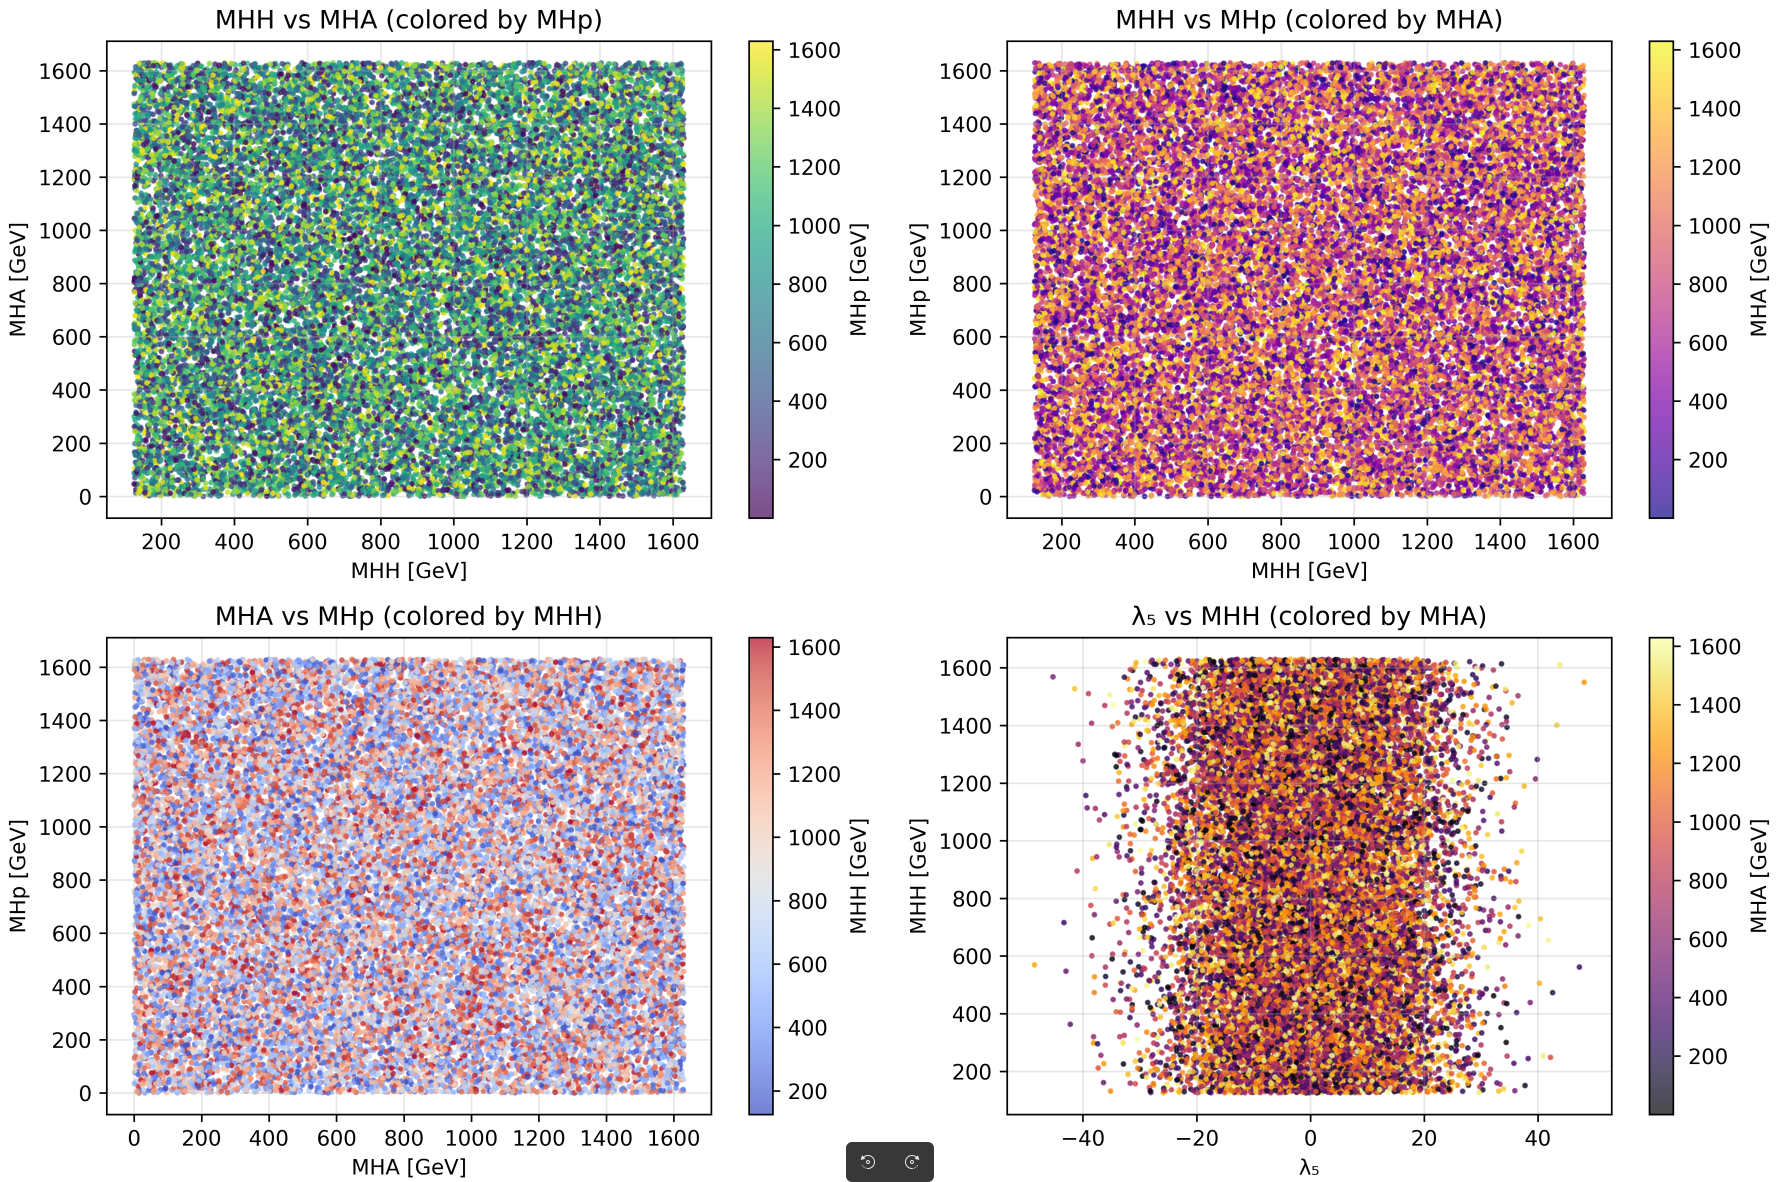
\includegraphics[width=\textwidth]{Initial_THDM_param_scan_analysis}
  \end{center}
\end{frame}


\section{Phenomenological Constraints}
\subsection{Theoretical Constraints}
\begin{frame}{{Vacuum Stability Constraints:}}
    The potential must be bounded from below at large field values.  

    \vfill
    The dominant quartic terms in the potential are:

    $$
    V_4 = \frac{\lambda_1}{2} X_1^4 + \frac{\lambda_2}{2} X_2^4 
    + \lambda_3 X_1^2 X_2^2 
    + \lambda_4 X_1^2 X_2^2 \rho^2
    + \lambda_5 X_1^2 X_2^2 \rho^2 \cos 2\theta .
    $$

    where the fields have been parametrized as

    $$
    \Phi_1^{\dagger} \Phi_1 = X_1^2, \quad 
    \Phi_2^{\dagger} \Phi_2 = X_2^2, \quad 
    \Phi_1^{\dagger} \Phi_2 = X_1 X_2 \rho \, \mathrm{e}^{i \theta} \quad \text{with} \quad 0 \leq \rho \leq 1 .
    $$
    \vfill
    Here, $\rho$ is the normalized magnitude of the inner product between $\Phi_1$ and $\Phi_2$, obtained from the Cauchy--Schwarz inequality:
    $$
    |\Phi_1^{\dagger} \Phi_2| \leq \sqrt{(\Phi_1^{\dagger} \Phi_1)(\Phi_2^{\dagger} \Phi_2)} \; \Rightarrow \; 
    \rho = \frac{|\Phi_1^{\dagger} \Phi_2|}{X_1 X_2} \in [0,1] .
    $$
    Geometrically, $\rho$ plays the role of the cosine of the angle between the two Higgs doublets in field space:
    $\rho = 1$ means they are aligned, while $\rho = 0$ means they are orthogonal.

    
    
\end{frame}

\begin{frame}%{Potential must be Bounded from Below, $V_4>0$}
    % Thus, 
    % $$
    % V_4 = \frac{\lambda_1}{2} X_1^4 + \frac{\lambda_2}{2} X_2^4 
    % + \lambda_3 X_1^2 X_2^2 
    % + \lambda_4 X_1^2 X_2^2 \rho^2
    % + \lambda_5 X_1^2 X_2^2 \rho^2 \cos 2\theta
    % $$
    $V_4$ must have a minimum for all directions in field space, i.e., for all $X_1, X_2 \geq 0$ and $\rho \in [0,1]$.
    \vfill
    
    The term with $\theta$ is $ \lambda_5 X_1^2 X_2^2 \rho^2 \cos 2\theta$. 
    \begin{itemize}
        \item If $\lambda_5 > 0$, the minimum occurs at $\cos\theta = -1$, 
        \item else if $\lambda_5 < 0$, the minimum occurs at $\cos\theta = 1$.
        \item In any case, the term becomes $-|\lambda_5| X_1^2 X_2^2 \rho^2$ at the minimum.
    \end{itemize}

    \pause
    At the minimum, the term with $\rho$ is $\left(\lambda_4 - |\lambda_5|\right) X_1^2 X_2^2 \rho^2$. 
    \begin{itemize}
        \item If $\lambda_4 - |\lambda_5| > 0$, the minimum occurs at $\rho = 0$, then
        \begin{equation}
            V_4 = \frac{\lambda_1}{2} X_1^4 + \frac{\lambda_2}{2} X_2^4 
            + \lambda_3 X_1^2 X_2^2
        \end{equation}
        and we require $\lambda_1 > 0$, $\lambda_2 > 0$, and $\lambda_3 + \sqrt{\lambda_1 \lambda_2} > 0$. \pause
        \item else if $\lambda_4 - |\lambda_5| < 0$, the minimum occurs at $\rho = 1$, then
        \begin{equation}
            V_4 = \frac{\lambda_1}{2} X_1^4 + \frac{\lambda_2}{2} X_2^4 
            + \left(\lambda_3 + \lambda_4 - |\lambda_5|\right) X_1^2 X_2^2
        \end{equation}
        and we require $\lambda_1 > 0$, $\lambda_2 > 0$, $\lambda_3' + \sqrt{\lambda_1 \lambda_2} > 0$, with $\lambda_3' = \lambda_3 + \lambda_4 - |\lambda_5|$.
    \end{itemize}
    
    

    \vfill
    In Summary, the bounded from below conditions are:
    $$\boxed{
    \lambda_1 > 0, \quad \lambda_2 > 0, \quad
    \lambda_3 + \sqrt{\lambda_1\lambda_2} > 0, \quad
    \lambda_3 + \lambda_4 - |\lambda_5| + \sqrt{\lambda_1\lambda_2} > 0.
    }
    $$
\end{frame}

\begin{frame}{$\lambda_1 > 0, \quad \lambda_2 > 0$ constraints}
  \begin{center}
    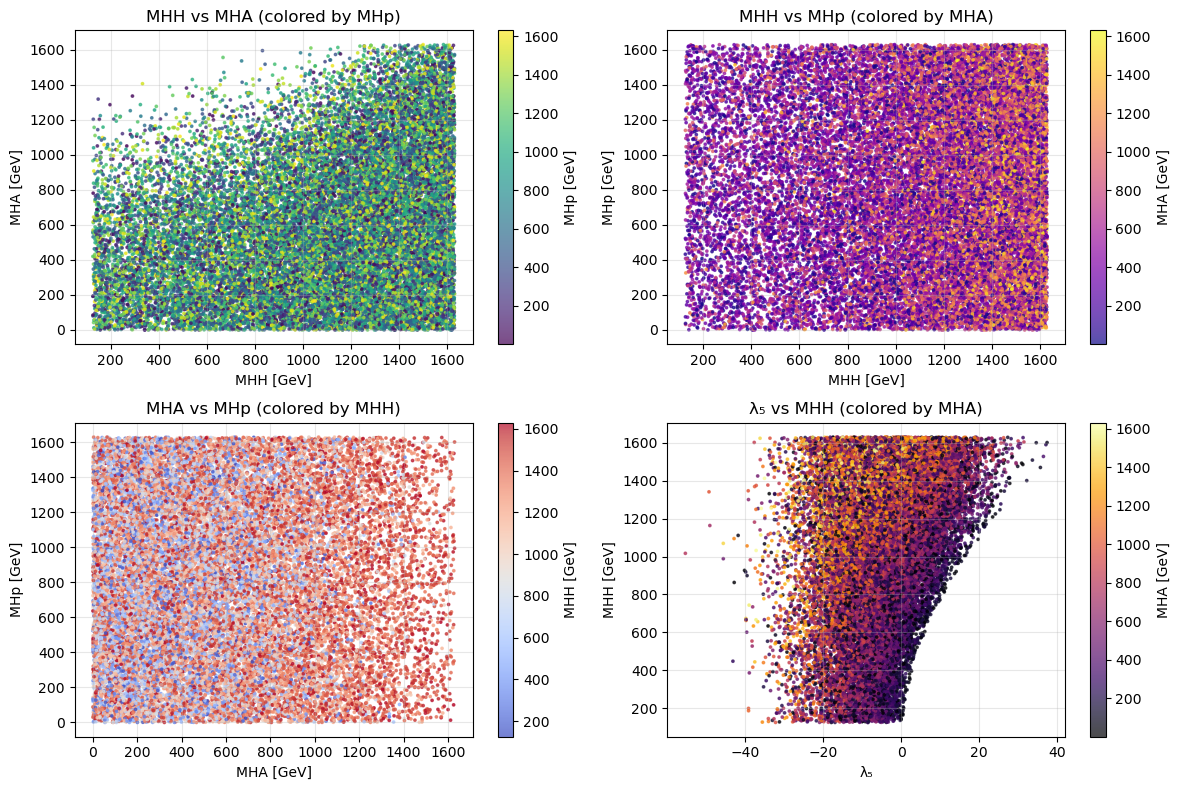
\includegraphics[width=\textwidth]{stability_lam1_2_condition_THDM_param_scan_analysis}
  \end{center}
\end{frame}


\begin{frame}{$\sqrt{\lambda_1\lambda_2} + \lambda_3 + \lambda_4 > \text{máx}(\lambda_4, \abs{\lambda_5})$}
  \begin{center}
    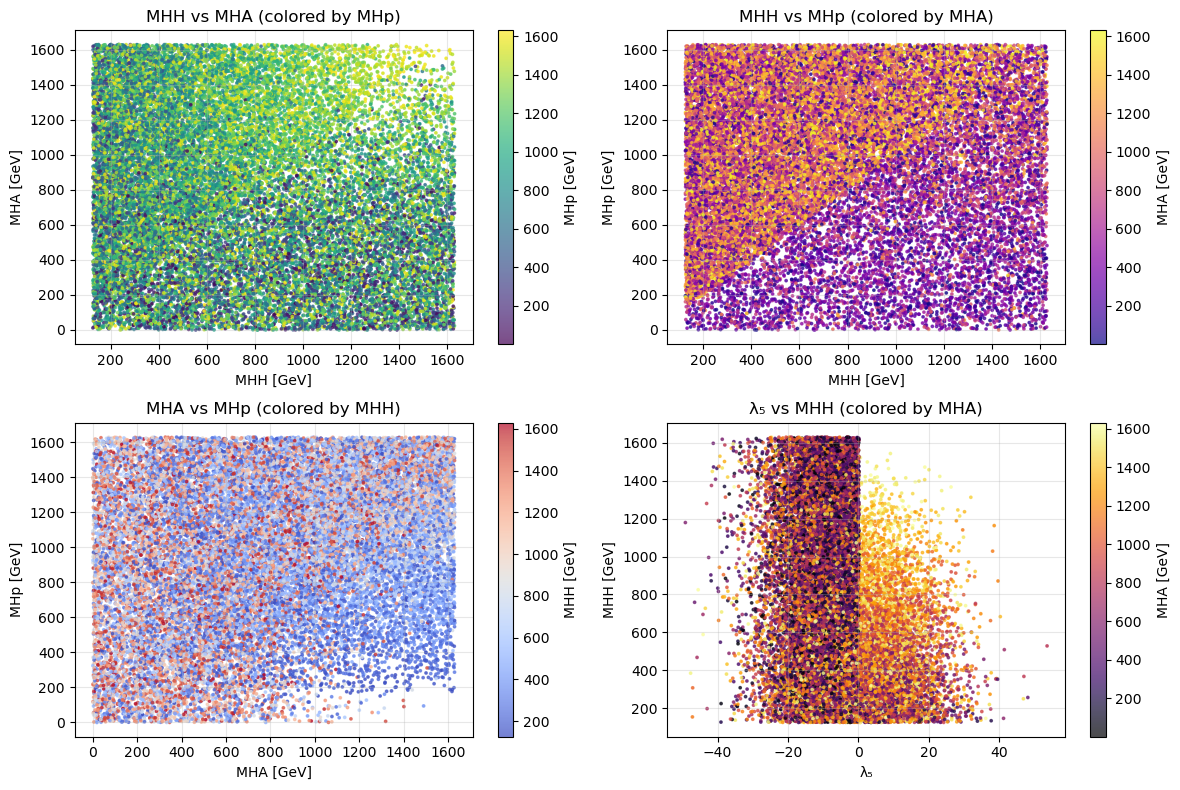
\includegraphics[width=\textwidth]{stability_lam3_4_condition_THDM_param_scan_analysis}
  \end{center}
\end{frame}

\begin{frame}{Bounded from Below Conditions}
    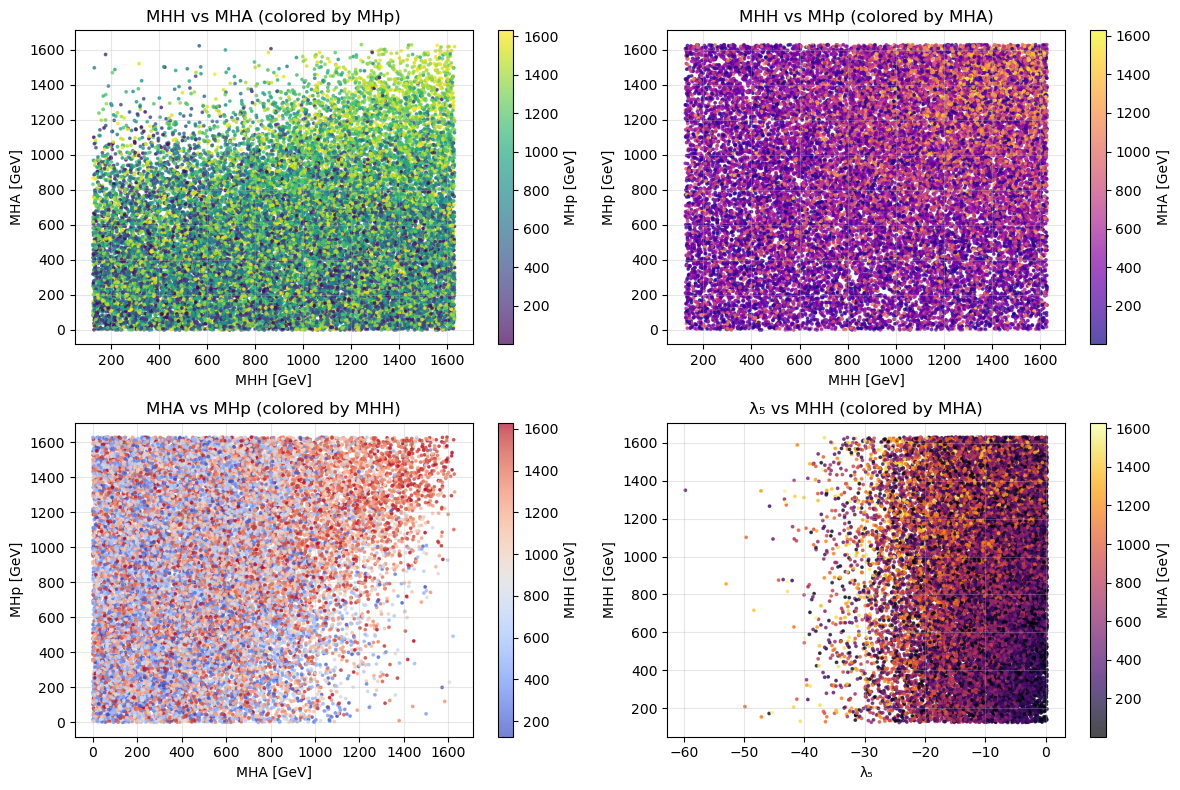
\includegraphics[width=\textwidth]{stability_lam1_2_3_4_condition_THDM_param_scan_analysis}
\end{frame}

\begin{frame}{Electroweak Vacuum Stability}

\begin{itemize}
    \item The scalar potential can have multiple minima - we must ensure our EW-breaking vacuum is the \textbf{global minimum}\vfill
    
    \item Metastability could lead to dangerous vacuum decay via quantum tunneling.\vfill
    
    \item To guarantee the selected vacuum is truly the lowest-energy state, we require:
    \begin{equation*}
    m_{12}^2\left(m_{11}^2 - k^2 m_{22}^2\right)\left(\tan\beta - k\right) > 0
    \end{equation*}
    where $k \equiv (\lambda_1/\lambda_2)^{1/4}$ compares the quartic couplings. \vfill

    \item The details of this condition requires a mapping of the potential as a Minkowskian manifold and stability of the Landau-Ginzburg effective potential is given in \cite{Barroso:2013awa}.
\end{itemize}

\end{frame}
\begin{frame}{Vacuum Stability Conditions}
  \begin{center}
    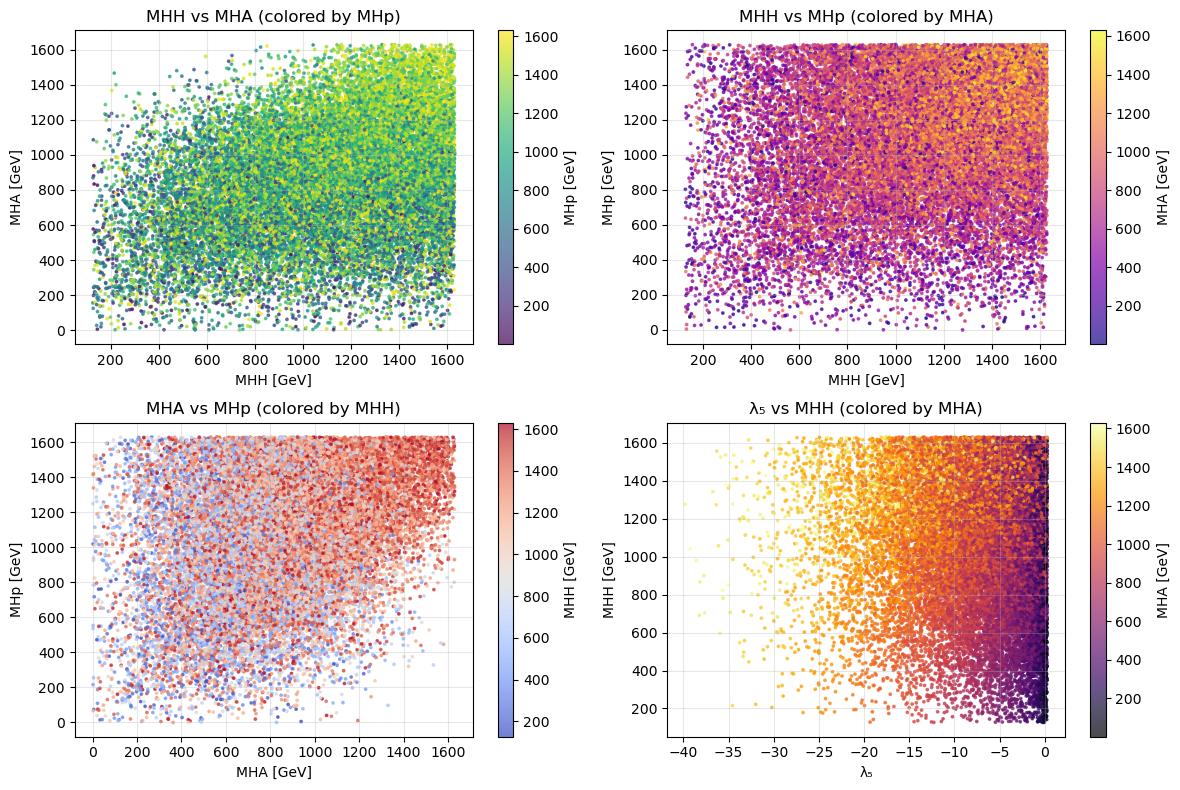
\includegraphics[width=\textwidth]{vacuum_stable_THDM_param_scan_analysis}
  \end{center}
    
\end{frame}

\begin{frame}{Unitarity Constraints}

From quantum mechanics, the S-matrix must be unitary:
\begin{equation*}
S = 1 + iT \quad \Rightarrow \quad T^\dagger T = -i(T - T^\dagger)
\end{equation*}
For scattering processes $s_1 s_2 \rightarrow s_3 s_4$, this implies bounds on amplitudes.\vfill 

The matrix element for the process is defined as:
\begin{equation*}
\langle\{s_1, s_2 \}|iT|\{s_3, s_4\}\rangle \equiv i\mathcal{M}\delta^4(k_3+k_4-p_1-p_2)(2\pi)^4
\end{equation*}

From the scattering theory, the amplitude $\mathcal{M}$ can be expaded in partial waves:
\begin{equation*}
\mathcal{M} = \sum_{J=0}^{\infty}(2J+1)a_J P_J(\cos\theta)
\implies
a_J \equiv \frac{1}{32 \pi} \sqrt{\frac{4\left|\mathbf{p}^{\text{in}}\right|\left|\mathbf{p}^{\text{out}}\right|}{2^{\delta_{12}} 2^{\delta_{34}} s}} \int_{-1}^1 d(x) \mathcal{M} P_J(x)
\end{equation*}
where $P_J$ are Legendre polynomials and $a_J$ are the partial wave amplitudes.

So, we have 
\begin{equation}
    -\frac{i}{2}\left(a_J-a_J^{\dagger}\right) \geq a_J a_J^{\dagger} 
    \implies
    \text{Re}(a_J) \leq \frac{1}{2}
\end{equation}
\end{frame}


\begin{frame}{Unitarity Constraints}
    At large energies, the dominant contributions are the spherically symmetric, $J=0$, partial wave amplitudes and $s\approx \abs{\mathbf{p}}^2$. Thus, 
    \begin{equation}
        \Re{a_0} \sim \frac{1}{16 \pi} \sqrt{2 ^{-\delta_{12}-\delta_{34}}} Q_{1234} \leq \frac{1}{2}
    \end{equation}
    where $Q_{1234} $ is the quartic coupling of the process $s_1 s_2 \rightarrow s_3 s_4$.


Considering all the possible processes, 
\begin{equation*}
|a_\pm|, |b_\pm|, |c_\pm|, |e_\pm|, |f_\pm|, |g_\pm| \leq 8\pi
\end{equation*}
where the eigenvalues are:
  {\small
  \begin{equation}
    \begin{aligned}
    a_{ \pm} & =\frac{3}{2}\left(\lambda_1+\lambda_2\right) \pm \sqrt{\frac{9}{4}\left(\lambda_1-\lambda_2\right)^2+\left(2 \lambda_3+\lambda_4\right)^2} &\mathrm{e}_{ \pm} & =\lambda_3+2 \lambda_4 \pm 3 \lambda_5 \\
    b_{ \pm} & =\frac{1}{2}\left(\lambda_1+\lambda_2\right) \pm \sqrt{\frac{1}{4}\left(\lambda_1-\lambda_2\right)^2+\lambda_4^2} & \mathrm{f}_{ \pm} & =\lambda_3 \pm \lambda_4 \\
    c_{ \pm} & =\frac{1}{2}\left(\lambda_1+\lambda_2\right) \pm \sqrt{\frac{1}{4}\left(\lambda_1-\lambda_2\right)^2+\lambda_5^2} & \mathrm{g}_{ \pm} & =\lambda_3 \pm \lambda_5
    \end{aligned}
  \end{equation}
  }
  \textbf{It is just a safety check, not the strict theory limitation.}
\end{frame}

\begin{frame}{Example: $\abs{f_+}=\abs{\lambda_3 + \lambda_4}\approx \left| m_h^2 + m_A^2 - m_{H}^2 \right|/v^2  < 8\pi$}
  \begin{center}
    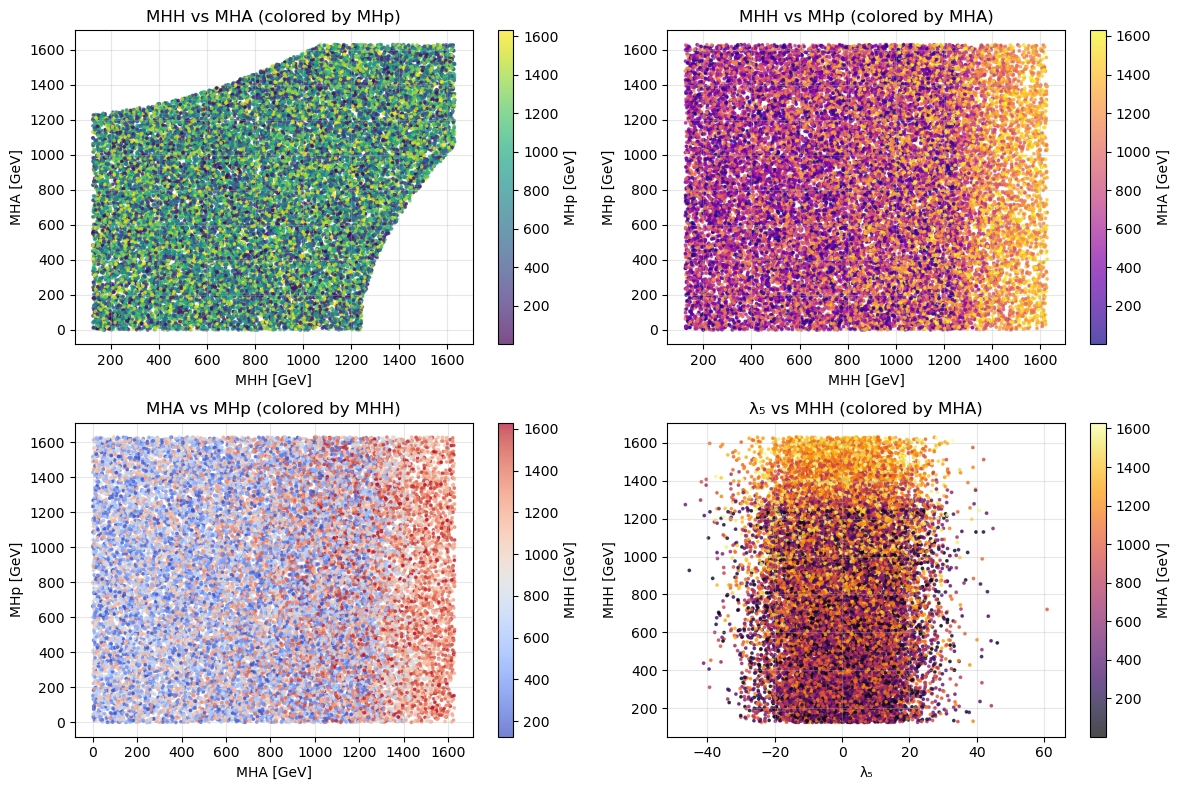
\includegraphics[width=\textwidth]{unitarity_f_plus_THDM_param_scan_analysis}
  \end{center}
    
\end{frame}

\begin{frame}{All Unitarity Constraints}
    \begin{center}
        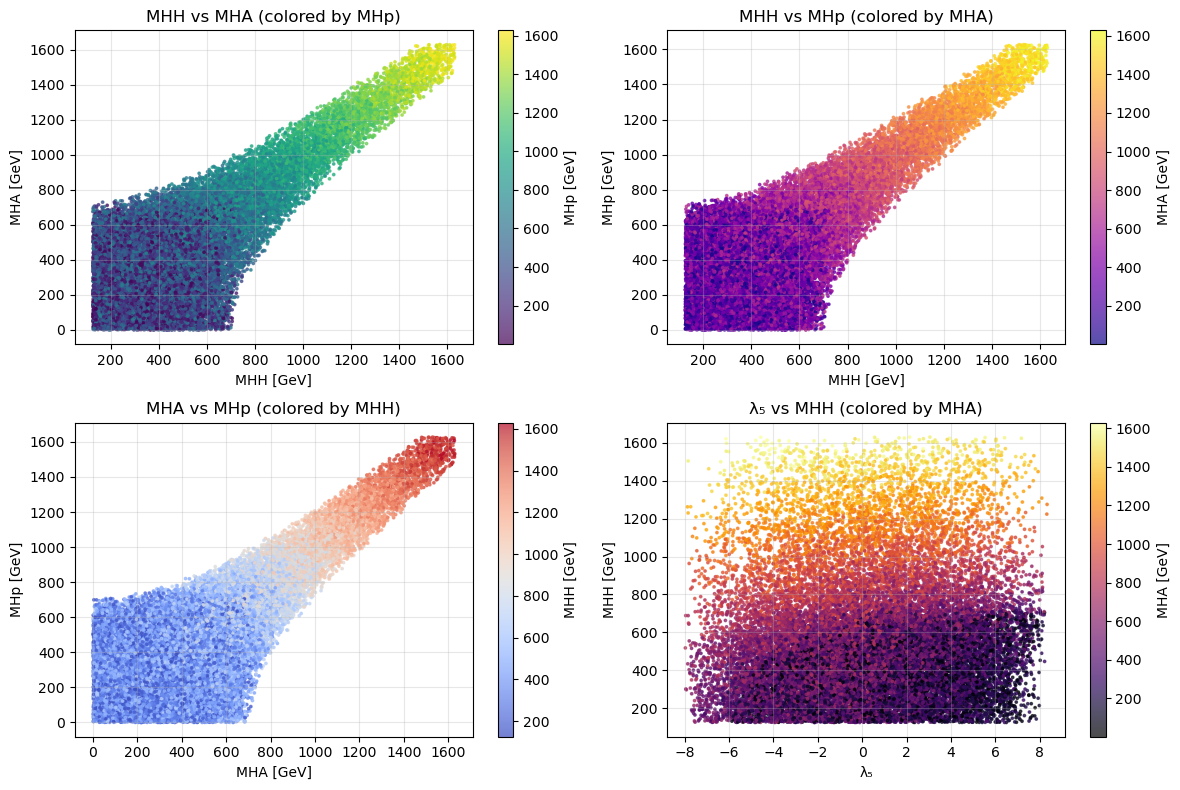
\includegraphics[width=\textwidth]{unitarity_satisfied_THDM_param_scan_analysis}
    \end{center}
\end{frame}

\begin{frame}{All the theoretical constraints}
    \begin{center}
        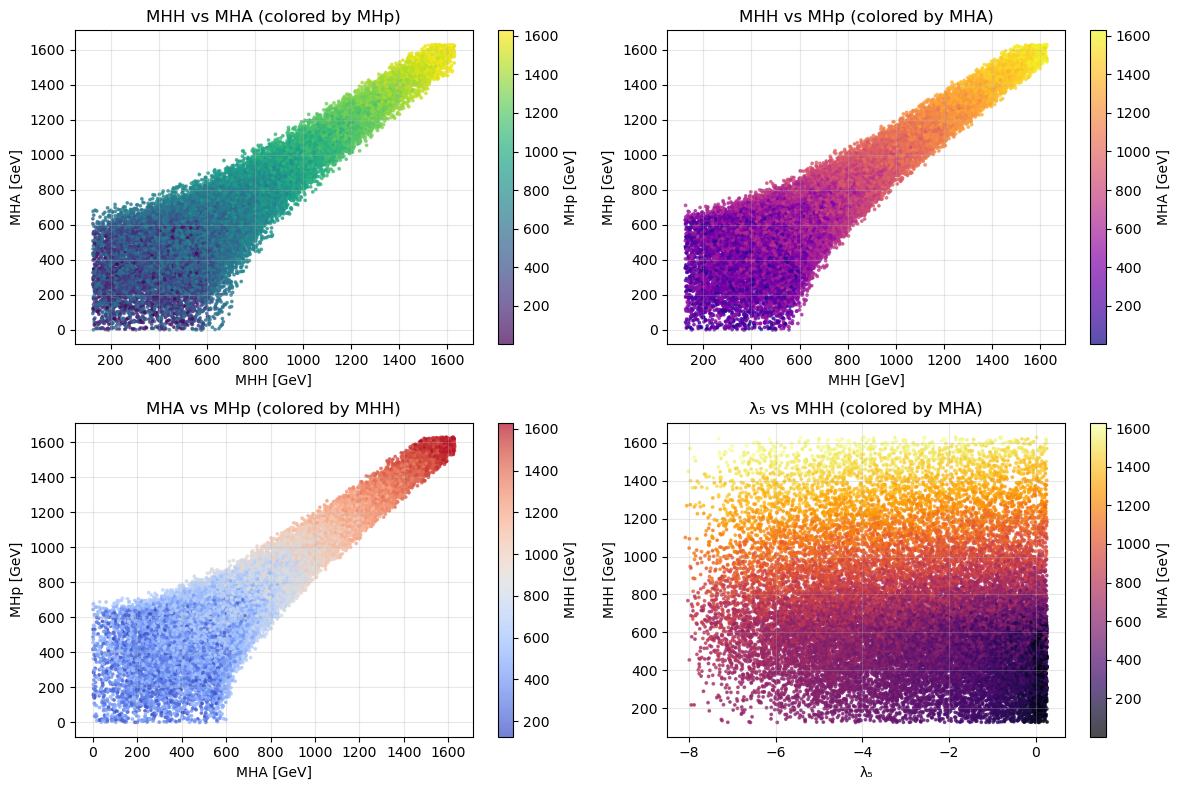
\includegraphics[width=\textwidth]{Theoretical_constraints_satisfied_THDM_param_scan_analysis}
    \end{center}
\end{frame}

\subsection{Experimental Constraints}
\begin{frame}{Oblique Parameters}

  $W$-boson mass at one-loop level could have small corrections to the mass:
  $$
  m_W^2=m_W^2(\mathrm{SM})+\frac{\alpha c_W^2}{c_W^2-s_W^2} m_Z^2\left(-\frac{1}{2} S+c_W^2 T+\frac{c_W^2-s_W^2}{4 s_W^2} U\right)
  $$
  This corrections are parametrized by the oblique parameters $S$, $T$, and $U$ which are complicated loop-function that we calculated in Spheno.
  \vfill
  The accuracy of the $W$ boson mass requires:
    \begin{align}
      S & = 0.02 \pm 0.10, \\
      T & = 0.07 \pm 0.12, \\
      U & = 0.00 \pm 0.09
    \end{align}
  These parameters are crucial for precision tests of the Standard Model and for constraining new physics scenarios.
\end{frame}

\begin{frame}{Oblique Parameters Constraints}
  \begin{center}
    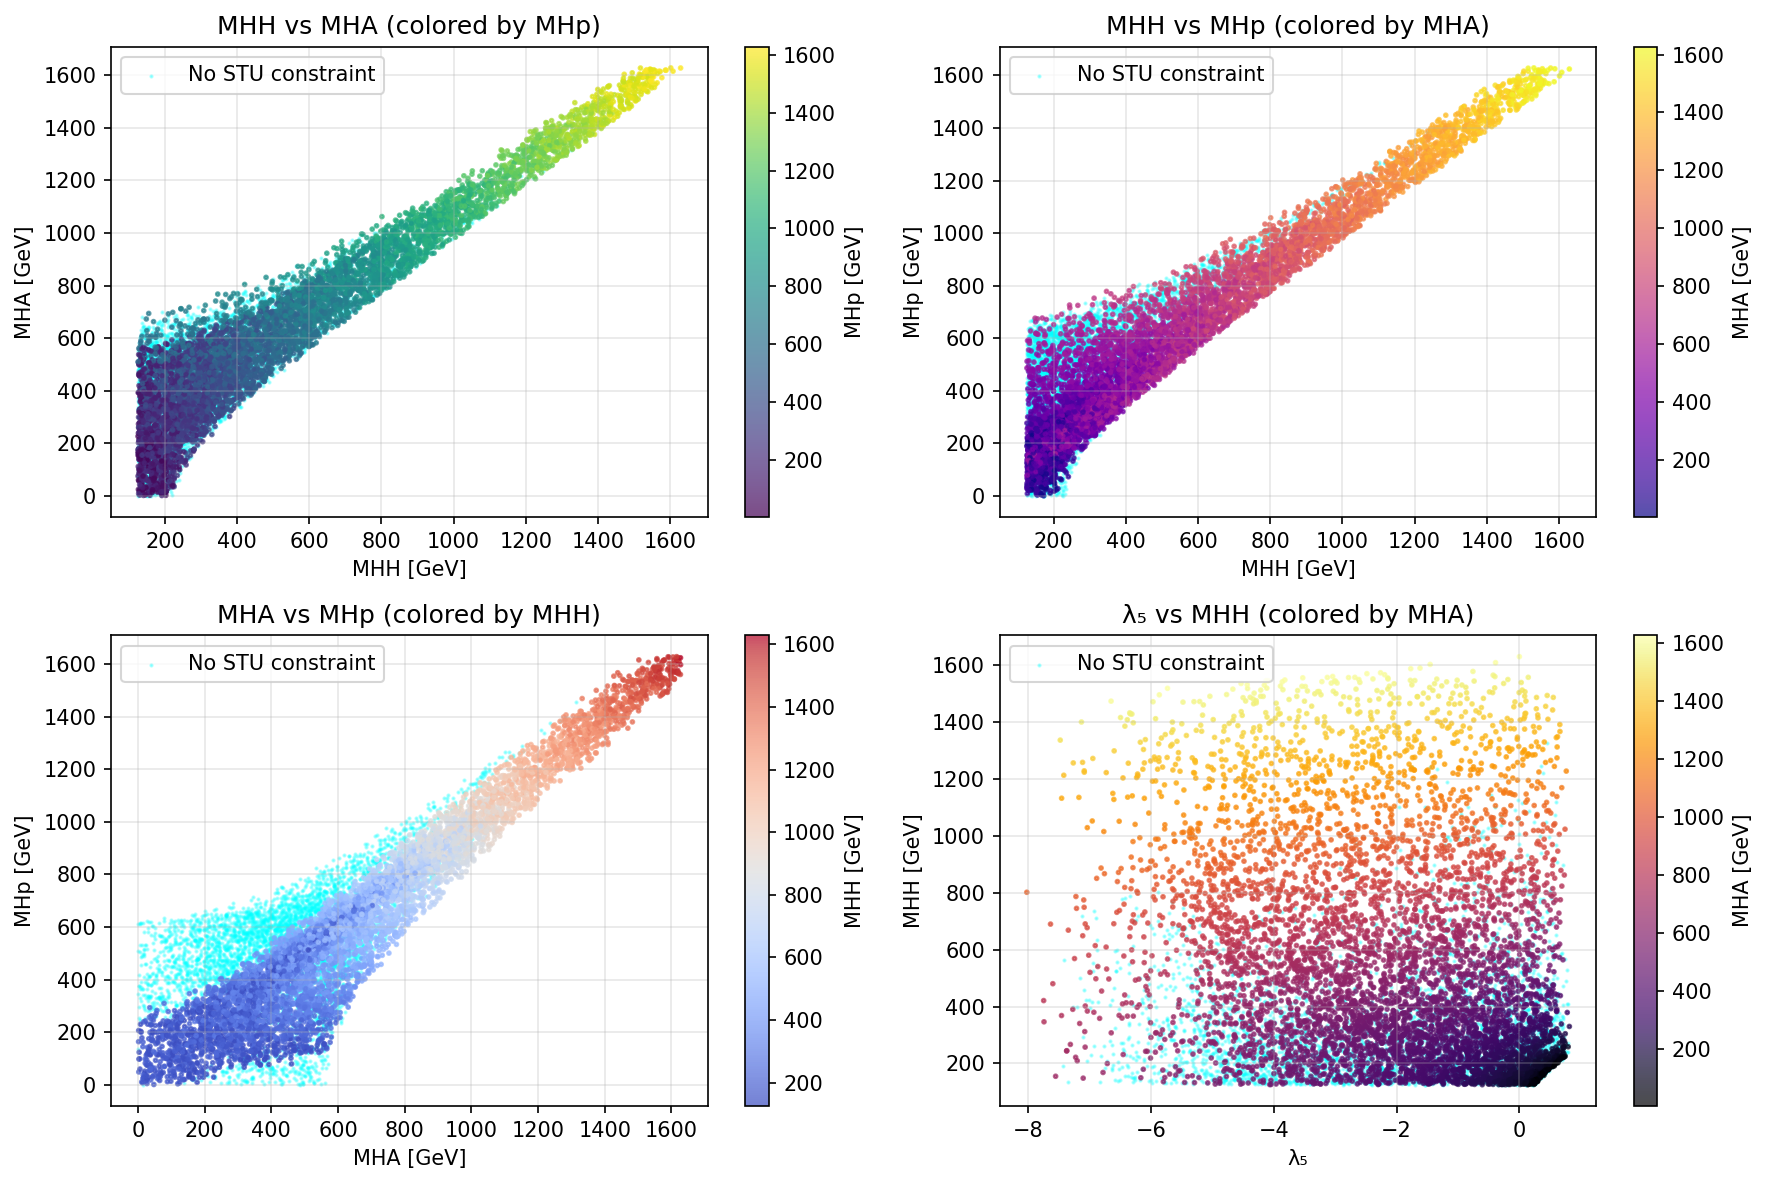
\includegraphics[width=\textwidth]{stu_THDM_param_scan_analysis}
  \end{center}
\end{frame}


\section{Yukawa Sector}
\subsection{FCNC-free Models}
\begin{frame}{Yukawa Sector}
    In order to suppress flavor-changing neutral currents (FCNCs), we impose a $\mathbb{Z}_2$ symmetry on the Yukawa sector resulting in four types of Yukawa interactions:
    \begin{center}
        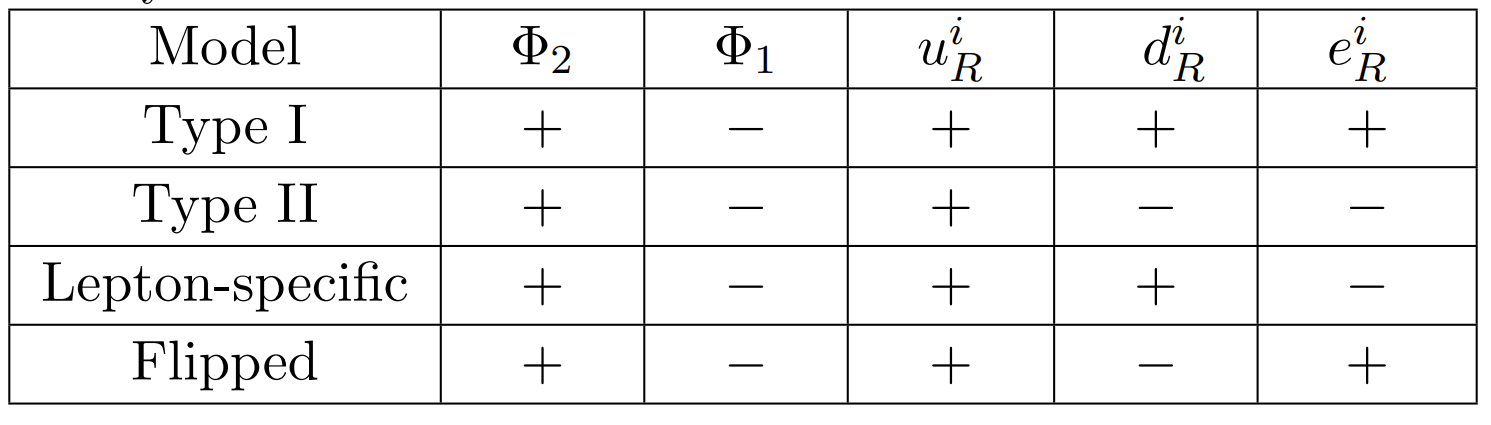
\includegraphics[width=0.75\textwidth]{Table_Z2_charges.png}
    \end{center}
    According to different charge assignments, there are four different models with Yukawa interactions:

    $$
    \begin{aligned}
    & -\mathcal{L}=Y_{u 2} \bar{Q}_L \tilde{\Phi}_2 u_R+Y_{d 2} \bar{Q}_L \Phi_2 d_R+Y_{\ell 2} \bar{L}_L \Phi_2 e_R+\text { h.c. }(\text { type I }), \\
    & -\mathcal{L}=Y_{u 2} \bar{Q}_L \tilde{\Phi}_2 u_R+Y_{d 1} \bar{Q}_L \Phi_1 d_R+Y_{\ell 1} \bar{L}_L \Phi_1 e_R+\text { h.c. }(\text { type II }), \\
    & -\mathcal{L}=Y_{u 2} \bar{Q}_L \tilde{\Phi}_2 u_R+Y_{d 1} \bar{Q}_L \Phi_2 d_R+Y_{\ell 1} \bar{L}_L \Phi_1 e_R+\text { h.c. }(\text { lepton specific }), \\
    & -\mathcal{L}=Y_{u 2} \bar{Q}_L \tilde{\Phi}_2 u_R+Y_{d 1} \bar{Q}_L \Phi_1 d_R+Y_{\ell 1} \bar{L}_L \Phi_2 e_R+\text { h.c. ( flipped model) },
    \end{aligned}
    $$

    where $Q_L^T=\left(u_L, d_L\right), L_L^T=\left(\nu_L, l_L\right), \widetilde{\Phi}_{1,2}=i \tau_2 \Phi_{1,2}^*$, and $Y_{u 2}, Y_{d 1,2}$ and $Y_{\ell 1,2}$ are $3 \times 3$ matrices in family space.
\end{frame}

\begin{frame}{Yukawa sector After EWSB}
    We can obtain the Yukawa couplings

    $$
    \begin{aligned}
    -\mathcal{L}_Y= & \frac{m_f}{v} y_h^f h \bar{f} f+\frac{m_f}{v} y_H^f H \bar{f} f \\
    & -i \frac{m_u}{v} \kappa_u A \bar{u} \gamma_5 u+i \frac{m_d}{v} \kappa_d A \bar{d} \gamma_5 d+i \frac{m_{\ell}}{v} \kappa_{\ell} A \bar{\ell} \gamma_5 \ell \\
    & +H^{+} \bar{u} V_{\mathrm{CKM}}\left(\frac{\sqrt{2} m_d}{v} \kappa_d P_R-\frac{\sqrt{2} m_u}{v} \kappa_u P_L\right) d+h . c . \\
    & +\frac{\sqrt{2} m_{\ell}}{v} \kappa_{\ell} H^{+} \bar{\nu} P_R e+h . c .
    \end{aligned}
    $$

    where $y_h^f=\sin (\beta-\alpha)+\cos (\beta-\alpha) \kappa_f$ and $y_H^f=\cos (\beta-\alpha)-\sin (\beta-\alpha) \kappa_f$. The values of $\kappa_u$, $\kappa_d$ and $\kappa_{\ell}$ for the four models are
    \begin{center}
        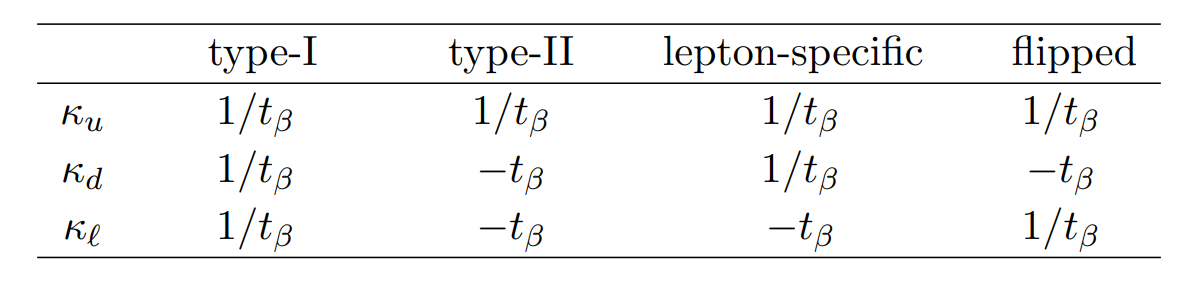
\includegraphics[width=0.75\textwidth]{Table_kappa.png}
    \end{center}
    These models naturally have preferential couplings to the third generation fermions, due to the Higgs Mechanism.
\end{frame}
\begin{frame}{$H^\pm$ Constraints}
    % The charged Higgs boson $H^\pm$ is similar to the $W^\pm$ vector bosons, and its phenomenology is similar to the $W$ one with important contributions on the third generation fermions.
    \begin{center}
        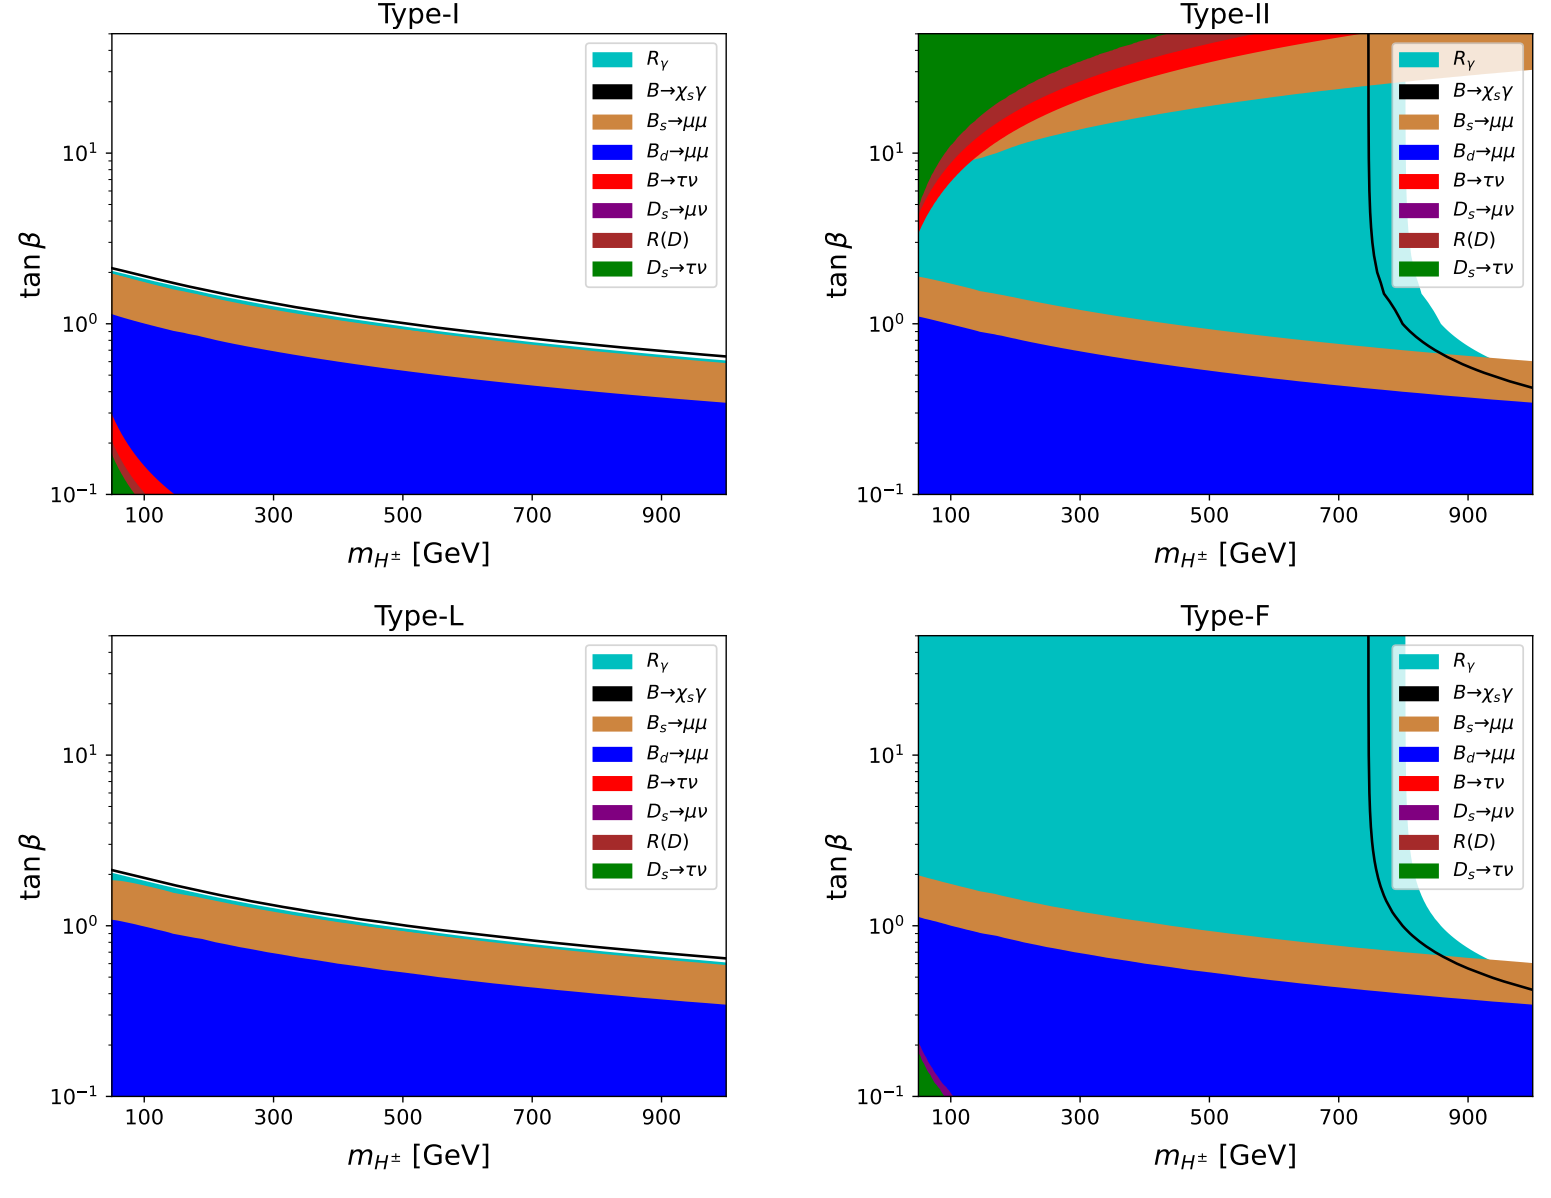
\includegraphics[width=0.92\textwidth]{Hpm_Constrains_by_Model.png}
    \end{center}
\end{frame}
\subsection{Phenomenology of the Type II THDM}
\begin{frame}{Phenomenology of the Type II THDM}
    We are interested in channels $\tau \tau$. As the heavy Higgs and the pseudoscalar have the structure
    $$
    \kappa_u=\frac{1}{\tan\beta}, \qquad \kappa_d=\kappa_\ell=\tan\beta,
    $$
    in the Yukawa sector for the Type II THDM, we have a enhancement of the $b$ and $\tau$ Yukawa couplings for large $\tan\beta$ values.\vfill

    That is why the {$H^\pm$ Constraints} are more stringent for the Type II THDM, leaving a allowed region starting at $m_{H^\pm} \gtrsim 800$ GeV, and $\tan\beta \in [1, 15]$.\vfill

    The contribution of the top-loop diagram of the gluon-gluon fusion process $gg \rightarrow H / A$ will be suppressed, meanwhile the contribution of the $b$-loop diagram will be enhanced, and the $b\bar b$ fusion become relevant for the production of the heavy Higgs boson $H$. 
    \vfill

    In the same way, the branching fraction of the $H/A \rightarrow \tau \tau$ decay channel will be enhanced for large $\tan\beta$ values, while the decay to top quarks will be suppressed.
\end{frame}

\begin{frame}{$H$ Constraints For Type II THDM}
    Using the software Higgs-Bounds 5, we can check the constraints on the heavy Higgs boson $H$. 
    \begin{center}
        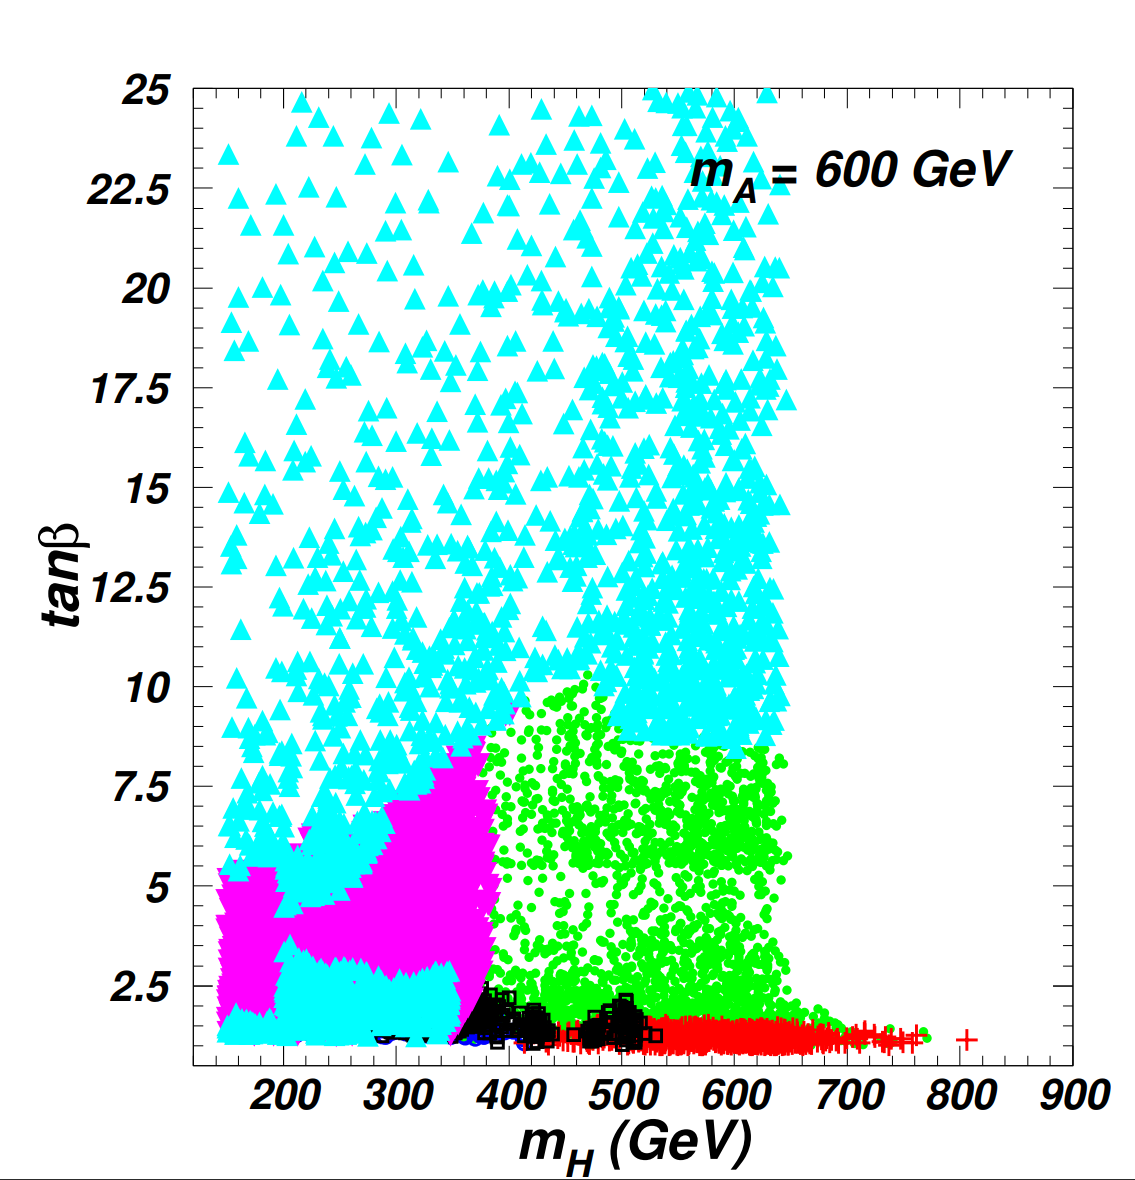
\includegraphics[width=0.48\textwidth]{HH_Constraints.png}
    \end{center}
    The triangles (sky blue), circles (royal blue), squares (black), inverted triangles (purple), and pluses (red) are respectively excluded by the $H / A \rightarrow \tau^{+} \tau^{-}, H \rightarrow W W, Z Z, \gamma \gamma, H \rightarrow h h, A \rightarrow H Z$, and $A \rightarrow h Z$ channels at the LHC. The bullets (green) samples are allowed by various LHC direct searches.
\end{frame}

\section{Final Remarks and Next Steps}
\begin{frame}{Summary}
    \begin{block}{Key Results from THDM Analysis}
        \begin{itemize}
            \item \textbf{Theoretical Framework:} Extended SM with two Higgs doublets $\Phi_1, \Phi_2$ 
            \begin{itemize}
                \item[$\rightarrow$] 5 physical scalars: $h$ (125 GeV), $H$, $A$, $H^\pm$ + 3 Goldstones
                \item[$\rightarrow$] Decoupling limit: $\cos(\beta-\alpha) \approx 0$ for SM-like behavior
            \end{itemize}
            
            \item \textbf{Constraints to the Scalar Potential:}
            \begin{itemize}
                \item[$\rightarrow$] Vacuum stability: $\lambda_1, \lambda_2 > 0$; $\sqrt{\lambda_1\lambda_2}+\lambda_3+\lambda_4 > \text{máx}(\lambda_4, \abs{\lambda_5})$ bounded-from-below conditions
                \item[$\rightarrow$] Unitarity: $|a_\pm|, |b_\pm|, |c_\pm|, |e_\pm|, |f_\pm|, |g_\pm| \leq 8\pi$
                \item[$\rightarrow$] EW precision: Oblique parameters $S$, $T$, $U$ within $1\sigma$
            \end{itemize}
            
            \item \textbf{Type II THDM Phenomenology:}
            \begin{itemize}
                \item[$\rightarrow$] Enhanced $\tau$, $b$ couplings: $\kappa_d = \kappa_\ell = \tan\beta$
                \item[$\rightarrow$] Suppressed top couplings: $\kappa_u = 1/\tan\beta$
                \item[$\rightarrow$] Strong $H^\pm$ constraints: $m_{H^\pm} \gtrsim 800$ GeV, $\tan\beta \in [1,15]$
            \end{itemize}
            
            \item \textbf{Experimental Constraints:}
            \begin{itemize}
                \item[$\rightarrow$] LHC searches exclude regions via $H/A \to \tau\tau$, $H \to WW/ZZ$
                \item[$\rightarrow$] Allowed parameter space identified for future studies
            \end{itemize}
        \end{itemize}
    \end{block}
    
    \begin{exampleblock}{Main Achievement}
        \centering
        Systematic parameter scan establishing \textbf{viable THDM Type II regions} \\
        consistent with all theoretical and experimental constraints
    \end{exampleblock}
\end{frame}

\begin{frame}{Next Steps}
    \begin{itemize}
        \item \textbf{Parameter Scan:} Perform a scan over the parameter space of the THDM, focusing on the Type II model with $\tan\beta$ values between 1 and 15 and $m_{H^\pm}$ starting from 800 GeV.\vfill
        \item \textbf{Performance improves:} Define a compressed mass region using a single mass parameter. \vfill
        \item \textbf{Collider Phenomenology:} check with higgs bounds the allowed points and constraints on the heavy Higgs boson $H$ and the pseudoscalar $A$ on the entire points that pass the preliminar steps from the scan. \vfill
        \item \textbf{Good Parameter Space:} Identify the good parameter space for the Type II THDM, to add further analysis.
    \end{itemize}
\end{frame}
\begin{frame}
    \begin{center}
        {\Huge Thank you for your attention!}
        
        \vfill
        
        {\Large Questions?}
        
        \vfill
        
        \textit{Details to be added based on specific analysis requirements}
    \end{center}
\end{frame}

% PRINT BIBLIOGRAPHY
\begin{frame}[allowframebreaks]{References}
    \printbibliography%[heading=none]
\end{frame}

\end{document}
